\documentclass[conference]{IEEEtran}
\IEEEoverridecommandlockouts
% The preceding line is only needed to identify funding in the first footnote. If that is unneeded, please comment it out.
\usepackage{cite}
\usepackage{amsmath,amssymb,amsfonts}
\usepackage{algorithmic}
\usepackage{graphicx}
\usepackage{textcomp}
\usepackage{xcolor}
\usepackage{float}

\floatstyle{boxed} 
\restylefloat{figure}

\def\BibTeX{{\rm B\kern-.05em{\sc i\kern-.025em b}\kern-.08em
    T\kern-.1667em\lower.7ex\hbox{E}\kern-.125emX}}
\begin{document}

\title{Detect Sleep States Using Accelerometers}

\author{
    \IEEEauthorblockN{Juan Carlos Quintero Rubiano}
    \IEEEauthorblockA{Code: 20232020172\\
    \textit{Systems Engineering} \\
    \textit{Francisco Jose de Caldas District University}\\
    Bogota, Colombia \\
    jcquineror@udistrital.edu.co}
    \and
    \IEEEauthorblockN{Nicolas Diaz Salamanca}
    \IEEEauthorblockA{Code: 20222020059\\
    \textit{Systems Engineering} \\
    \textit{Francisco Jose de Caldas District University}\\
    Bogota, Colombia \\
    jndiazs@udistrital.edu.co}
    \and
    \centering 
    \IEEEauthorblockN{Juan Felipe Wilches Gomez}
    \IEEEauthorblockA{Code: 20232020---\\
    \textit{Systems Engineering} \\
    \textit{Francisco Jose de Caldas District University}\\
    Bogota, Colombia \\
    }
}

\maketitle

\begin{abstract}
This workshop is a systemic analysis of the prized competition of Kaggle, which consists of a system that detects
sleep states using accelerometers. The system is designed to analyze the data collected from accelerometers and
classify different sleep states based on the patterns observed in the data. The analysis includes a detailed examination
of the system's components, their interactions, and the emergent behaviors that emerges from these interactions.
By understanding the system's dynamics, we aim to identify potential areas for improvement and optimization, 
ultimately enhancing the accuracy and reliability of sleep state detection.
\end{abstract}

\begin{IEEEkeywords}
Systemic analysis, sleep state detection, accelerometers, emergent behaviors, optimization.
\end{IEEEkeywords}

\section{Introduction}
\subsection{Competition Overview}

This workshop analyzes the Kaggle competition "Child Mind Institute - Detect Sleep States", which aims to improve sleep monitoring through accelerometer data analysis. The competition focuses on developing a model to accurately detect sleep onset and wakefulness using wrist-worn accelerometer data. This has the potential to enable larger-scale sleep studies and improve our understanding of sleep's impact on mood, behavior, and overall health, especially in children.

\subsubsection{Competition Objective}
The primary objective is to create a robust model for detecting sleep states from accelerometer data. This involves classifying periods of sleep and wakefulness by analyzing time-series data from wearable sensors. The model should generalize well across individuals and account for variations in sleep patterns to provide insights into sleep and potential sleep disorders. Ultimately, the goal is to improve awareness and guidance surrounding the importance of sleep.

\subsubsection{Dataset Structure}
The dataset consists of around 500 multi-day recordings of accelerometer data, labeled with sleep onset and wake events. The goal is to detect these events using time-series data from wrist-worn accelerometers.

Key components include:

\begin{itemize}
    \item \textbf{Accelerometer Data:} Located in \texttt{train\_series.parquet} and \texttt{test\_series.parquet}, containing \texttt{series\_id}, \texttt{step}, \texttt{timestamp}, \texttt{anglez}, and \texttt{enmo} columns.
    \item \textbf{Sleep Event Labels:} Found in \texttt{train\_events.csv}, providing sleep logs with \texttt{series\_id}, \texttt{night}, \texttt{event} (onset or wakeup), \texttt{step}, and \texttt{timestamp}.
\end{itemize}

\textbf{Important Considerations for Sleep Data:}
\begin{itemize}
    \item Sleep periods must be at least 30 minutes long and can have interruptions of activity no longer than 30 minutes.
    \item Only the longest sleep window each night is recorded.
    \item If no valid sleep window is found, no events are recorded.
    \item Periods of device removal (indicated by little signal variation) are not annotated.
\end{itemize}

\section{Systemic Analysis}
\subsection{Inputs Description}
\begin{itemize}
    \item \textbf{series id:} Unique identifier assigned to each data series, allowing differentiation between records from different sessions or devices.
    \item \textbf{step:} Represents the sequence or interval at which data is captured, facilitating the tracking of temporal progression during data collection.
    \item \textbf{timestamp:} A time marker that indicates the exact moment when each measurement was taken, essential for synchronizing and analyzing data over time.
    \item \textbf{anglez:} Represents the angular measure along the Z-axis, used to assess the device's orientation or tilt during data capture.
    \item \textbf{enmo:} A derived measure of acceleration that quantifies the magnitude of movement, crucial for detecting patterns and variations in activity that may be related to sleep states.
\end{itemize}

\subsection{System Components}
The system consists of several components that interact with each other to achieve the goal of detecting sleep states. These components include:
\begin{itemize}
    \item \textbf{Data Processor:} This component is responsible for cleaning, transforming, and preparing the accelerometer data for analysis. It includes tasks such as filtering noise, normalizing data, and extracting relevant features.
    \item \textbf{Event Detection:} This component identifies sleep onset and wake events based on the processed accelerometer data. Compare the data to classify the data into different sleep states.
    \item \textbf{States} Are 2 possible classification of the data, sleep and wakefulness. The system must be able to classify the data into these two states based on the patterns observed in the accelerometer data.
    \item \textbf{Sleep Duration Calculator} This component calculates the duration of sleep based on the detected sleep events. It helps in understanding the overall sleep patterns and their impact on health.
    \item \textbf{Pattern Recognizer} This component analyzes the detected sleep states and identifies patterns in the data. It helps in understanding the relationship between sleep states and various factors such as mood, behavior, and health.
    \item \textbf{Validator} This component validates that the detected sleep states correspond to the longest recorded sleep window.
\end{itemize}

\subsection{Components interactions}
\begin{enumerate}
    \item \textbf{Inputs} sends raw data to the \textbf{Data Processor}.
    \item \textbf{Data Processor} provides cleaned signals to \textbf{Event Detection}.
    \item \textbf{Event Detection} classifies data into \textbf{States}.
    \item \textbf{States} send sleep/wake up data to the \textbf{Sleep Duration Calculator}.
    \item \textbf{Sleep Duration Calculator} provides sleep periods to the \textbf{Pattern Recognizer}.
    \item \textbf{Pattern Recognizer} sends the sleep period to the \textbf{Validator} to confirm it corresponds to the longest recorded sleep window.
    \item If the validation fails, the \textbf{Validator} requests a new data sequence from \textbf{Event Detection}.
    \item If validation succeeds, the \textbf{Pattern Recognizer} sends the event and its score to the \textbf{output}.
\end{enumerate}

\subsection{Outputs}
A structured data file, typically in CSV format, containing a time series of detected sleep events (sleep onsets and awakenings) 
and associated confidence scores, facilitating further analysis and validation. The CSV file follows the next format:
\begin{table}[ht]
    \caption{Data output expected format} 
    \centering 
    \begin{tabular}{c c c c c} % centered columns (4 columns)
    \hline
    Row id & Series id & Step & Event & Score \\ [0.5ex] 
    \hline
    0 & 038441c925bb & 100 & onset & 0.0 \\
    1 & 038441c925bb & 105 & wakeup & 0.0 \\
    2 & 03d92c9f6f8a & 80 & onset & 0.5 \\ [1ex]
    \hline
    \end{tabular}
    \end{table}
\subsection{Diagram}
\begin{figure}[H]
    \centering
    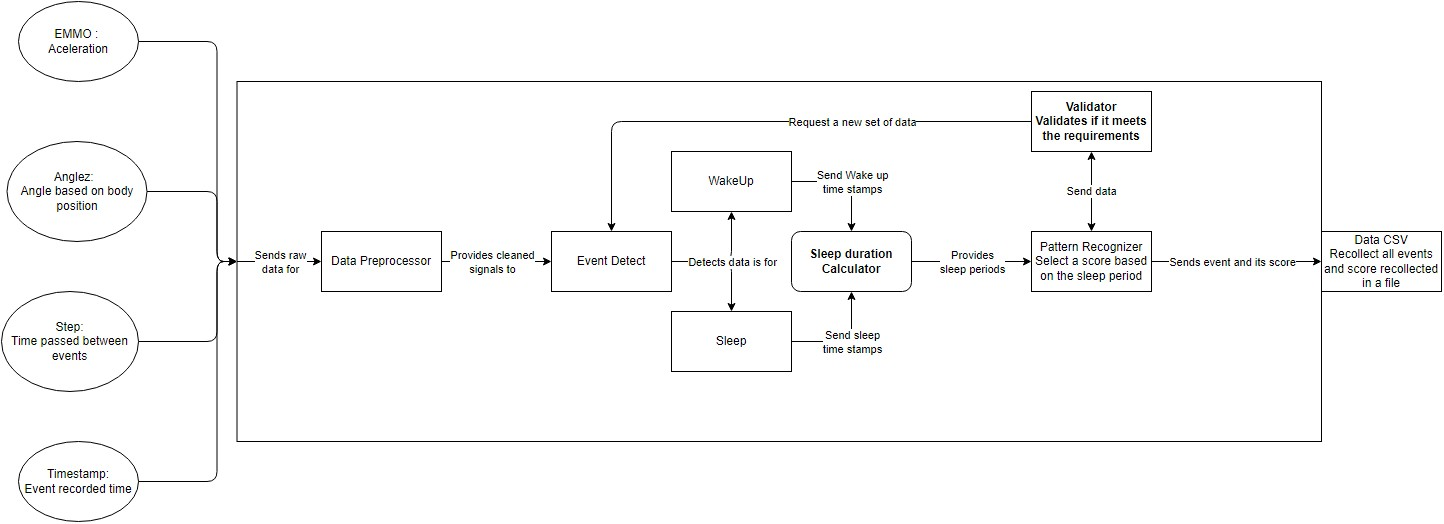
\includegraphics[width=\linewidth]{Workshop-1.JPG}
    \caption{System Diagram}
\end{figure}

\section{Chaos and randomness}
Chaos in a system refers to sensitivity to initial conditions.
A chaotic system is deterministic, meaning similar inputs should produce similar outputs; however,
the behavior of the system may change radically over time with small changes in the initial conditions,
making the system unpredictable.

In the context of the Child Mind Institute - Detect Sleep States competition, the elements and their relationships
in the sleep data collected from accelerometers can be viewed as chaotic parts of the system. External data collection
during sleep can be influenced by various factors such as sleep disorders, environmental conditions, and individual differences.
The main elements that interact with this chaos are fundamental to keeping disorder out of the system by
determining the different states of sleep and wakefulness as distinct categories. Without these elements, this complexity would make it
challenging to predict sleep states accurately.

Another important source of entropy within the system itself is the event detection component. When classifying accelerometer data into sleep states,
the algorithm must make decisions based on patterns that may not always be clear-cut.
This decision-making process introduces entropy as the boundary between sleep and wakefulness isn't always distinct in the data. Additionally,
the validation mechanism creates another layer of uncertainty when determining whether a detected sleep period is indeed the longest valid window.
These inherent decision points add entropy to the system's behavior even when the external inputs remain consistent.

\section{Complexity and sensitivity}
The proposed system is not expected to be complex due to the reduced number of relations per element. However, the feedback 
loop that emerges between the Event Detection, Sleep Duration Calculator, Pattern Recognizer, and Validator elements is sensitive to 
external chaos introduced by the variability in individual sleep patterns and inaccuracies in sensor measurements. 

The components of the system, such as Event Detection, Pattern Recognizer, and Validator, are sensitive to changes in their attributes. The entire system is vulnerable because if any element
fails to detect a sleep state accurately, it can lead to incorrect classifications and affect the overall performance of the system.
These factors can amplify the complexity of the system, requiring robust algorithms and validation mechanisms to ensure accurate
detection of sleep states and to avoid false positives or negatives that could loop infinitely in the feedback loop and register incorrect
data.

\section{Conclusions}

Secuential system:
Each component of the system depends on the proper funtioning of the previous one. This makes sure that the process runs in and orderly manner without interruptions.

Feedback:
The system incorporates an internal cycle that allows to detect posible errors as the data is processed. If a failure is identified, the analysis is repeated since the beggining to correct it.

Fault-Tolerant System:
In case of data loss or erroneus processing, the system includes a validator that detects the issue and restarts the cicle from the event detection phase, ensuring that errors do not affect the final result.

Data filter mechanism:
To prevent the entry of erroneus or irrelevant data, the system uses a filtering mechanism that closes the inputs under specific conditions, ensuring that only valid data is processed.

\subsection{Weaknesses}

\begin{itemize}
    \item \textbf{Falta de adaptacion a usuarios especificos:} The sleep pattern diagnosis of the program can be rendered unusable if the user suffers from any condition or takes medication that affects sleep patterns.
    \item \textbf{Dependence on the correct functioning of the validation:} The feedback cycle being complex it requires reliable algorithms and mechanisms of validation, causing the abscence of these to generate false positives or negatives.  
    \item \textbf{Infinite loops:} If the validation detects an error in the recieved data that can not be fixed during event detection it enters a loop where the erroneus validation is repeated.
    \item \textbf{Sensitivity to chaos:} The system is vulnerable to the randomness and the environment, like abrupt changes of sleep patterns or errors in the accelerometers. 
\end{itemize}

\end{document}
